8. La figura 1 , se representa un diagrama $PV$ simplificado del ciclo de gas ideal de Joule. Todos los procesos son cuasi-estáticos y $\mathrm{C_P}$ es constante. Demuestre que la eficiencia térmica de un motor que realiza este ciclo es
$$
\eta=1-\left(\frac{P_{\mathbf{1}}}{P_2}\right)^{(\gamma-1) / \gamma}
$$
figura 1. Ciclo de gas ideal Joule

\begin{figure}[h]
    \centering
    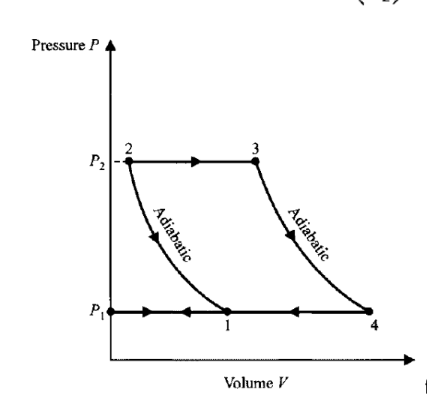
\includegraphics[width=0.5\textwidth]{diagrama.png}
    \label{fig:figura1}    
\end{figure}